\documentclass[12pt, letterpaper]{article}
\usepackage[margin=1in]{geometry}
\usepackage[utf8]{inputenc}
\usepackage{amsmath}
\usepackage{listings}
\usepackage{graphicx} 
\usepackage{fancyhdr}
\usepackage{booktabs} % For formal tables
\usepackage{float}
\usepackage{hyperref}
\usepackage{indentfirst}
\usepackage{multicol}
\usepackage{bookmark}
\usepackage[T1]{fontenc}
\usepackage{inconsolata}
\usepackage{listings}
\usepackage{color}
\usepackage{xcolor}

\renewcommand{\baselinestretch}{0.9}
\renewcommand{\rmdefault}{ptm}

\pagestyle{fancy}
\fancyhf{}
\setlength{\headheight}{15pt}
\rhead{Nicholas Quandt}
\lhead{McMaster Add-In for Autodesk Inventor}
\rfoot{Page \thepage}


\definecolor{bluekeywords}{rgb}{0.13,0.13,1}
\definecolor{greencomments}{rgb}{0,0.5,0}
\definecolor{redstrings}{rgb}{0.9,0,0}
\lstdefinestyle{sharpc}{language=[Sharp]C,
showspaces=false,
showtabs=false,
breaklines=true,
showstringspaces=false,
breakatwhitespace=true,
escapeinside={(*@}{@*)},
commentstyle=\color{greencomments},
keywordstyle=\color{bluekeywords},
stringstyle=\color{redstrings},
basicstyle=\ttfamily,
frame=lr,
rulecolor=\color{blue!80!black}
}

\begin{document}
\begin{titlepage}
   \begin{flushright}
       \vspace*{5cm}
 
       {\Huge \textbf{Design Document}}
 
       \vspace{0.5cm}
        McMaster-Carr Add-In for Autodesk Inventor\\
        Version 1.0.4 $\bullet$ December 07 2019
 
       \vspace{1.5cm}
 
       \textbf{Nicholas Quandt}
       \\
       nicholas.quandt@marquette.edu
       \vfill
       Marquette University Masters Student of\\
       Computational Mathematical and Statistical Sciences\\
       \vspace{1cm}
 
   \end{flushright}
\end{titlepage}

\section{Overview}
This project aims to implement an embedded web-browser into Autodesk Inventor 2019 \cite{Inventor}. The purpose being 
to allow a user to browse the McMaster-Carr online catalog of products, in order to eventually
include a product within their Inventor files \cite{McMaster}. Nearly every product in the catalog has a 3D model
available for download, along with properties pertaining to the part. The McMaster Add-In for Autodesk Inventor (MAFI)
will reduce time needed to implement these 3D models into an Inventor project.
\section{Context}
This docuemnt should give a user or other developer ample knowledge of the current state of MAFI, including
software packages implemented, code repositories, and languages used, along with goals for the future, challenges faced, etc.
\subsection{Document Conventions and Definitions}
The following describes all naming conventions used throughout the document:
\begin{itemize}
    \item MAFI: The McMaster-Carr Add-In for (Autodesk) Inventor software.
    \item Inventor: The computer application "Autodesk Inventor 2019" developed by Autodesk, Inc. \cite{Inventor}.
    \item McMaster: The online catalog available at www.mcmaster.com \cite{McMaster}.
    \item API: Application programming interface.
    \item 3D model: A three dimensional representation of a physical object, as shown within a computer program such as Inventor.
    \item Add-in: A software that relies on a parent application in order to execute, typically embedded within the parent application, i.e. non-standalone.
    \item IProperties: A set of attributes embedded within each Inventor file such as part number, description and physical material.
    \item Button: A user interface element that executes a process of an application from a mouse click.
    \item .NET: A software framework developed by Microsoft that includes a large class library and provides language interoperability across several programming languages \cite{NET}.
    \item CefSharp: A fast, fully embedded web browser for .NET applications \cite{CEFSharp}.
\end{itemize}
\section{Scope}
MAFI is an application add-in built for Inventor as a method for more efficiently connecting to and retrieving models from, the 
McMaster database of 3D models that often are used by mechanical designers. 
It will allow for a, direct, in-program access to the online catalog. Along with, "fast" conversion of 
the database file-type (.stp) into something usable by an Inventor user (.ipt). This is a software that should speed 
up design projects for engineers who use 3D models available from McMaster, in their Inventor projects.
\section{Overview of Requirements}
These requirements are a summary of the user stories gathered from the developer and potential users of the add-in. See Appendix A
for a collection of user stories.
\begin{enumerate}
\item Runs in Windows 64-bit for Inventor 2019 software.
\item Use Inventor API to add Button for interface.
\item Use McMaster online catalog that has links to 3d models of the majority of their items. Primarily hardware, fasteners, etc.
\item Best to keep online interface from McMaster, and somehow open the "form" in inventor to access.
\item Replace "add to cart" button in HTML with "add to assembly" or "open as part" buttons.
\end{enumerate}
\newpage
\section{Languages and Packages}
\begin{multicols}{2}

\begin{itemize}
    \item C\#
    \item XAML
    \item HTML
    \item Autodesk Inventor Interop 2020
    \item CEFSharp v69.0 \cite{CEFSharp}
    \item .NET 4.7.2 \cite{NET}
\end{itemize}
\end{multicols}

\section{User Interface}
\begin{figure}[H]
    \centering
    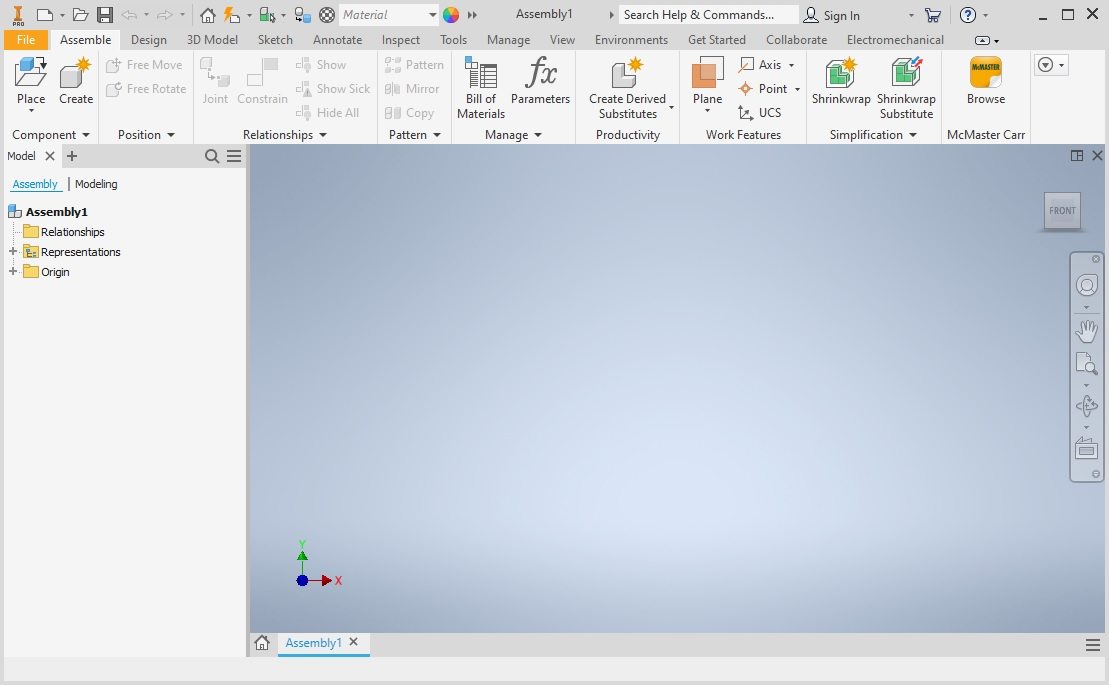
\includegraphics[width=0.7\textwidth]{Figures/mcMasterButton.JPG}
    \caption{The button(far right) addition to the ribbon interface within Autodesk Inventor.}
\end{figure}
\begin{figure}[H]
    \centering
    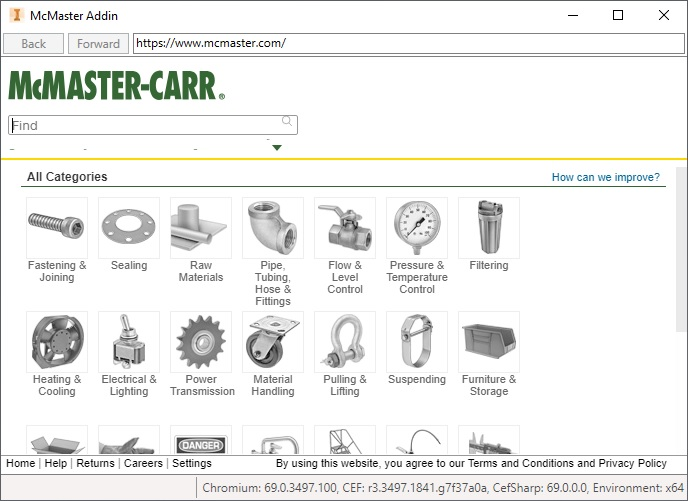
\includegraphics[width=0.7\textwidth]{Figures/webBrowserView.jpg}
    \caption{The browser instance following the button execute event.}
\end{figure}
\begin{figure}[H]
    \centering
    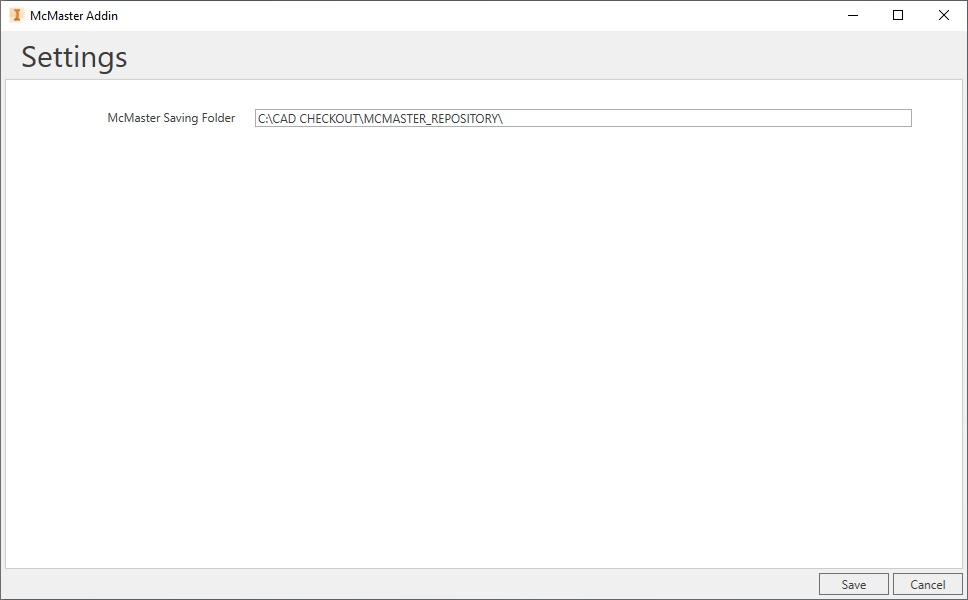
\includegraphics[width=0.7\textwidth]{Figures/webBrowserSettings.jpg}
    \caption{The settings page for the Add-In.}
\end{figure}
\begin{figure}[H]
    \centering    
    \begin{minipage}{0.6\textwidth}
        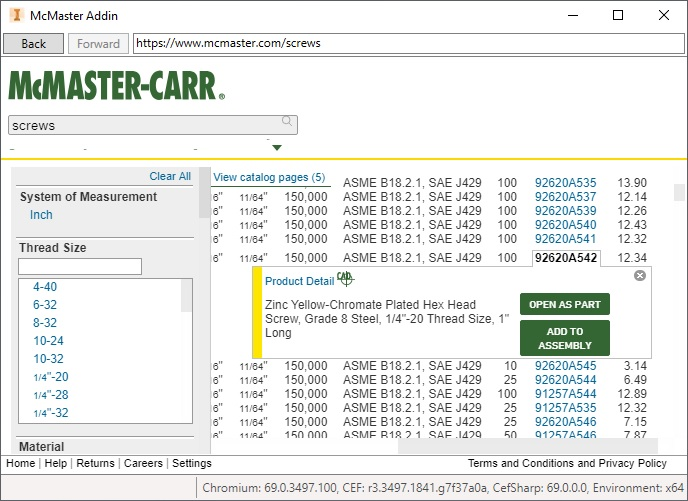
\includegraphics[width=0.9\textwidth]{Figures/webBrowserNewButtons.jpg}
    \end{minipage}
    \begin{minipage}{0.2\textwidth}
        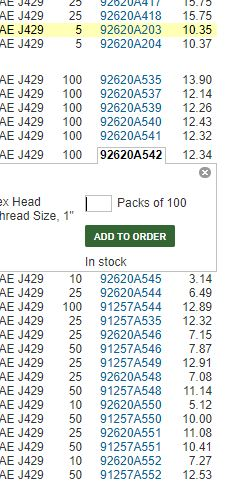
\includegraphics[width=0.9\textwidth]{Figures/webBrowserOld.JPG}
    \end{minipage}
    \caption{The alteration of the McMaster webpage for new model saving interactions(new on left, old on right)}
\end{figure}
\newpage
\section{Classes}
\subsection{StandardAddInServer}
This class is responsible for all Add-In initialization, such as hooking into the primary application 
and calling for a new instance of the McMasterButton to be added into
the ribbon interface within Inventor. Currently it contains the method GetSource() as well which 
stores webpage html to memory in order to parse for a file location, of which can be returned to an instance of 
the McMasterImporter class for conversion from a .stp file to .ipt, something Inventor can work with. In 
order to obtain the html from a dynamically created javascript enabled webpage, an instance of HeadlessWebBrowser is
used to render the webpage silently.
\subsection{HeadlessWebBrowser}
This class is a background process version of the CefSharp utility. It allows for a silent operation of visiting 
webpages. This enables the software to obtain the html of the "part" page, which contains the url of the 3D model 
location.
\subsection{McMasterButton}
This class is a template for the button that StandardAddInServer adds to the Inventor interface. Upon 
clicking the button, an embedded web-browser will be open, MainWindow, to allow for a user to browse 
the McMaster catalog for a part they wish to obtain the 3D model of.
\subsection{MainWindow}
The MainWindow class is essentially a form that acts as a holder for MainView class and SettingsView class.
\subsection{MainView}
This class is the primary interface a user will see while using MAFI. The McMasterButton will create an 
instance of this web-browser form. Javascript is injected into the web-browser that dynamically adds "Open 
as Part" and "Add to Assembly" buttons within the webpage, See Appendix B/addButtonScripts.js for code that is ran via the chromium embedded browser. 
Clicking these buttons will execute methods to begin 
the importing process, which is handled by the McMasterImporter, owned by the StandardAddInServer. This class also contains a button 
for opening the SettingsView class UI.
\subsection{SettingsView}
The SettingsView class allows for the user to edit the add-in config file via a set of text boxes. It includes a save and cancel button, both of which return to the MainView. 
\subsection{McMasterImporter}
This class locates the Inventor translator feature that allows for .stp to .ipt conversion. Then when called 
will silently convert a file that was obtained from the McMaster catalog, from MainWindow.
\subsection{JavaScriptInteractionObj}
This class is a binding object that is sent from the MainView class to the CefSharp chromium webbrowser as a new javascript object. It allows for callbacks to the .NET underlying application. Essentially 
this class allows for the new buttons on the McMaster webpage to call to the add-in.
\section{Extra Notes}
\begin{itemize}
    \item CEFSharp v69.0 specifically. v69.0 is built into Inventor 2020, though .WPF package is not, so that may need to be included in release of .dll's, unless it can be embedded.
    \item Possible revisions after all other features:
    \begin{itemize}
        \item Take product information from online catalog and automatically import into Inventor part file.
        \item Implement a bill of materials export to send all McMaster items onto clipboard with appropriate QTY per assembly.
        \item Incorporate a "no model" warning for items that do not have corresponding 3d models.
        \item Option for choosing folder to save models per project, or per item.
        \item Always on top windowing, currently can end up behind, which leads to difficulties.
        \item Comments throughout code for future revising, if ever McMaster online changes.
        \item If final release available, contact McMaster to check usability, possible copyright or anything legal. 
        \item Possibly develop for use with Solidworks, a similar program by  Dassault Systèmes.
    \end{itemize}
    \item Current Issues:
    \begin{itemize}
        \item Web browser seems to lag on initial startup.
        \item During testing, there were cases of crashing while importing. Possibly a threading error.
    \end{itemize}
\end{itemize}
\section{References}
\begingroup
\renewcommand{\section}[2]{}
\bibliography{srs}
\bibliographystyle{IEEEtran}
\endgroup
\newpage
\section{Appendix A: Story Cards}
\begin{itemize}
    \item [101] As a user I want to be able to use Windows operating system.\\
    Acceptance Criteria: Runs on Windows 64-bit without errors.
    \item [102] As a user I want to use Autodesk Inventor 2020.\\
    Acceptance Criteria: Uses Autodesk Inventor 2020 without errors.
    \item [103] As a user I want to have access to McMaster-Carr catalog from within Inventor.\\
    Acceptance Criteria: No outside browser needed to access catalog, embed chromium into Inventor.
    \item [104] As a user I don't want the interface to change much.\\
    Acceptance Criteria: Uses original McMaster webpage layout, and original Inventor UI, except for new button.
    \item [105] As a user I should be able to add parts from McMaster right into my project.\\
    Acceptance Criteria: No outside program or steps needed to import file, all done via Inventor, or windows, in background.
    \item [106] As a user I want to be able to choose whether to add a part to my current
    assembly or as an individual part.\\
    Acceptance Criteria: Two individual buttons for "Add to Assembly" and "Open as Part".
    \item [107] As a user I would like properties like the material added to my file for me.\\
    Acceptance Criteria: Properties are auto-populated on file addition.
    \item [108] As a user I would like to have control over the saving location of files imported from McMaster.\\
    Acceptance Criteria: Incorporate a settings page/config file, for the addin that allows for options such as saving location, file naming conventions.
    \item [109] As a developer I would like to use C\# \\
    Acceptance Criteria: All code written with C\# on .NET 4.7.2 or newer
    \item [110] As a developer I shouldn't need to install too many files or packages on the final computer.\\
    Acceptance Criteria: Keep total file count below 3.
    \item [111] As a developer I should well document code to allow for future updates.\\
    Acceptance Criteria: An outside individual can proof read code and follow along without difficulty.
\end{itemize}

\newpage
\section{Appendix B: Code}
All code can be found on the MAFI github repository\cite{MAFI}.\\
StandardAddInServer.cs
\lstset{style=sharpc,caption={}}
\lstinputlisting{../McMasterAddin/McMasterAddin/StandardAddInServer.cs}
\newpage
HeadlessWebBrowser.cs
\lstinputlisting{../McMasterAddin/McMasterAddin/HeadlessWebBrowser.cs}
\newpage
McMasterButton.cs
\lstinputlisting{../McMasterAddin/McMasterAddin/McMasterButton.cs}
\newpage
MainWindow.xaml.cs
\lstinputlisting{../McMasterAddin/McMasterAddin/MainWindow.xaml.cs}
\newpage
McMasterImporter.cs
\lstinputlisting{../McMasterAddin/McMasterAddin/McMasterImporter.cs}
\newpage
MainView.xaml.cs
\lstinputlisting{../McMasterAddin/McMasterAddin/MainView.xaml.cs}
\newpage
SettingsView.xaml.cs
\lstinputlisting{../McMasterAddin/McMasterAddin/SettingsView.xaml.cs}
\newpage
addButtonScripts.cs
\lstinputlisting{../McMasterAddin/McMasterAddin/Resources/addButtonScripts.js}
\end{document}